\section{The Architecture of the HELIO infrastructure}
%(2 pages Motivation for the architecture adopted, duality of web services, how it fits together. 2 pages Gab Pieratoni to lead, 
%Donal and Marco to assist) 

\subsection{Goals and Contraints}
% 1/2 a page with the goals and constraints of the architecture. It should be linked with the previous section as it should explain
% how the aims of HELIO are served by the architecture.

The requirements of the Heliophysics community drove the design of the architecture, these have been formalized in the following set of guidelines:

\begin{itemize}
\item{\emph{Service Duality}. The HELIO services should be used both as part of the HELIO project and as ''standalone services''. This requirement imposed a decoupling layer in the access service layer so that the services themselves are not tied to any particular 
user interface or workflow engine}
\item{\emph{Workflow Agnosticism}. Although HELIO now uses Taverna (TODO: Donal: Add references to Taverna), it should \emph{in principle} support different workflows engines.}
\item{\emph{Need to Know policy}. The system should be simple to use for the scientific community, thus hiding from the users all the implementation details that are not strictly necessary.}
\item{\emph{Policy Compliance}. The system must respect the policies (whenever and wherever present) of the back ends used by the HELIO services.}
\item{\emph{Flexible Deployment}. The various HELIO services should be able to be instantiated in multiple copies and located in order to allow different optimization profiles.}
\end{itemize}

To achieve the Need to know policy, HELIO is based on a multy-layered Service Oriented Architecture (TODO: Marco: Any reference on SOA ? ) where information
flows are contained as much as possible within different layers. These different abstractions layer also de-couple the services from the workflow engine and the graphical user interface as dictated by the Workflow Agnosticism and Service Duality guidelines.
Policy Compliant is achieved by a Community Interaction Service that differentiates between different user's profiles and Flexible Deployment is possible by the use of specific services (The Registry and Monitoring Services) that list and monitor all the 
different instances of the services deployed within the HELIO infrastructure.

\subsection{Architecture}

Figure~\ref{arch.overview} shows the different layers of the HELIO architecture and the related information flows. 

\begin{figure}[!t]
\centering
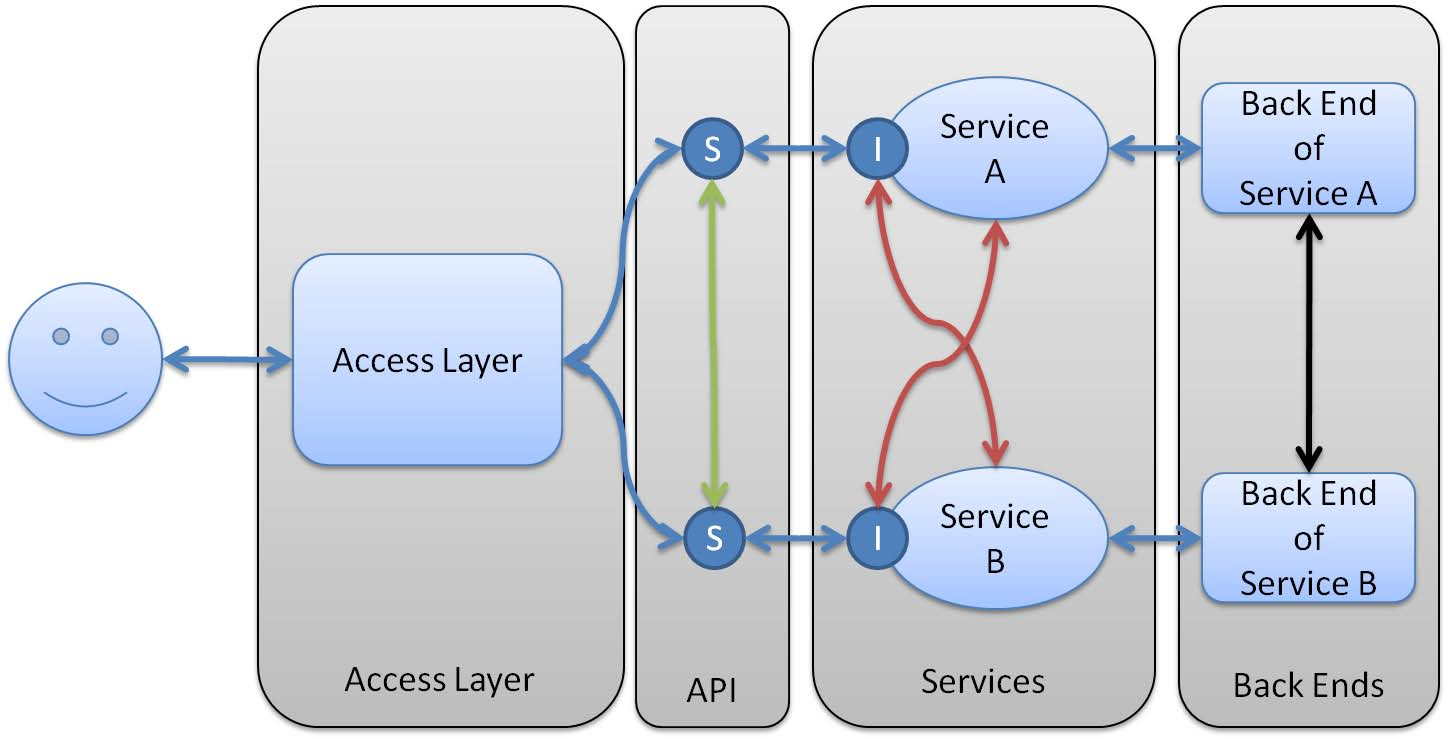
\includegraphics[width=3in]{HELIO-Architecture-Overview.pdf}
\caption{Overview and Information Flows in HELIO}
\label{arch.overview}
\end{figure}

The information flows are of two main kinds, there are \emph{vertical} flows within each layer and \emph{horizontal} flows that connect the different layers.
The vertical information flows connect some of the back ends (this is particularly true for the Processing and Storage Services). More frequently, the HELIO services
interact directly with each other as some of the stubs of the services do within the API.
One of the requirements of HELIO was that users may access the services in a variety of ways such as a local instance of Taverna Desktop, through a 
centralized Graphical User Interface called \emph{HFE} (Helio Front End) and user defined scripts. To define all these access modalities, the HELIO
architecture has a layer called \emph{Access Layer}, an abstraction that defines all the different modalities with which the users can connet to the services.

Figure~\ref{arch.detail} details the different components of the \emph{Access Layer} and their interactions. Users can connect to a centralized Graphical User Interface that uses an instance of the TAVERNA server.
Users can also use a local instance of a TAVERNA desktop to define workflows or can access directly the services through java or IDL (TODO: Bob, Andre: References to IDL) code.
Finally, some of the services, also offer standalone graphical user interfaces that offer advanced functionalities not available in the HFE.
  
The architecture of HELIO of Figure~\ref{arch.detail} also comprehends the HELIO API (further detailed in section~\ref{arch.api} and instances of the TAVERNA server and the TAVERNA desktop. The interactions between HELIO and TAVERNA are 
further detailed in section~\ref{arch.taverna} 

\begin{figure}[!t]
\centering
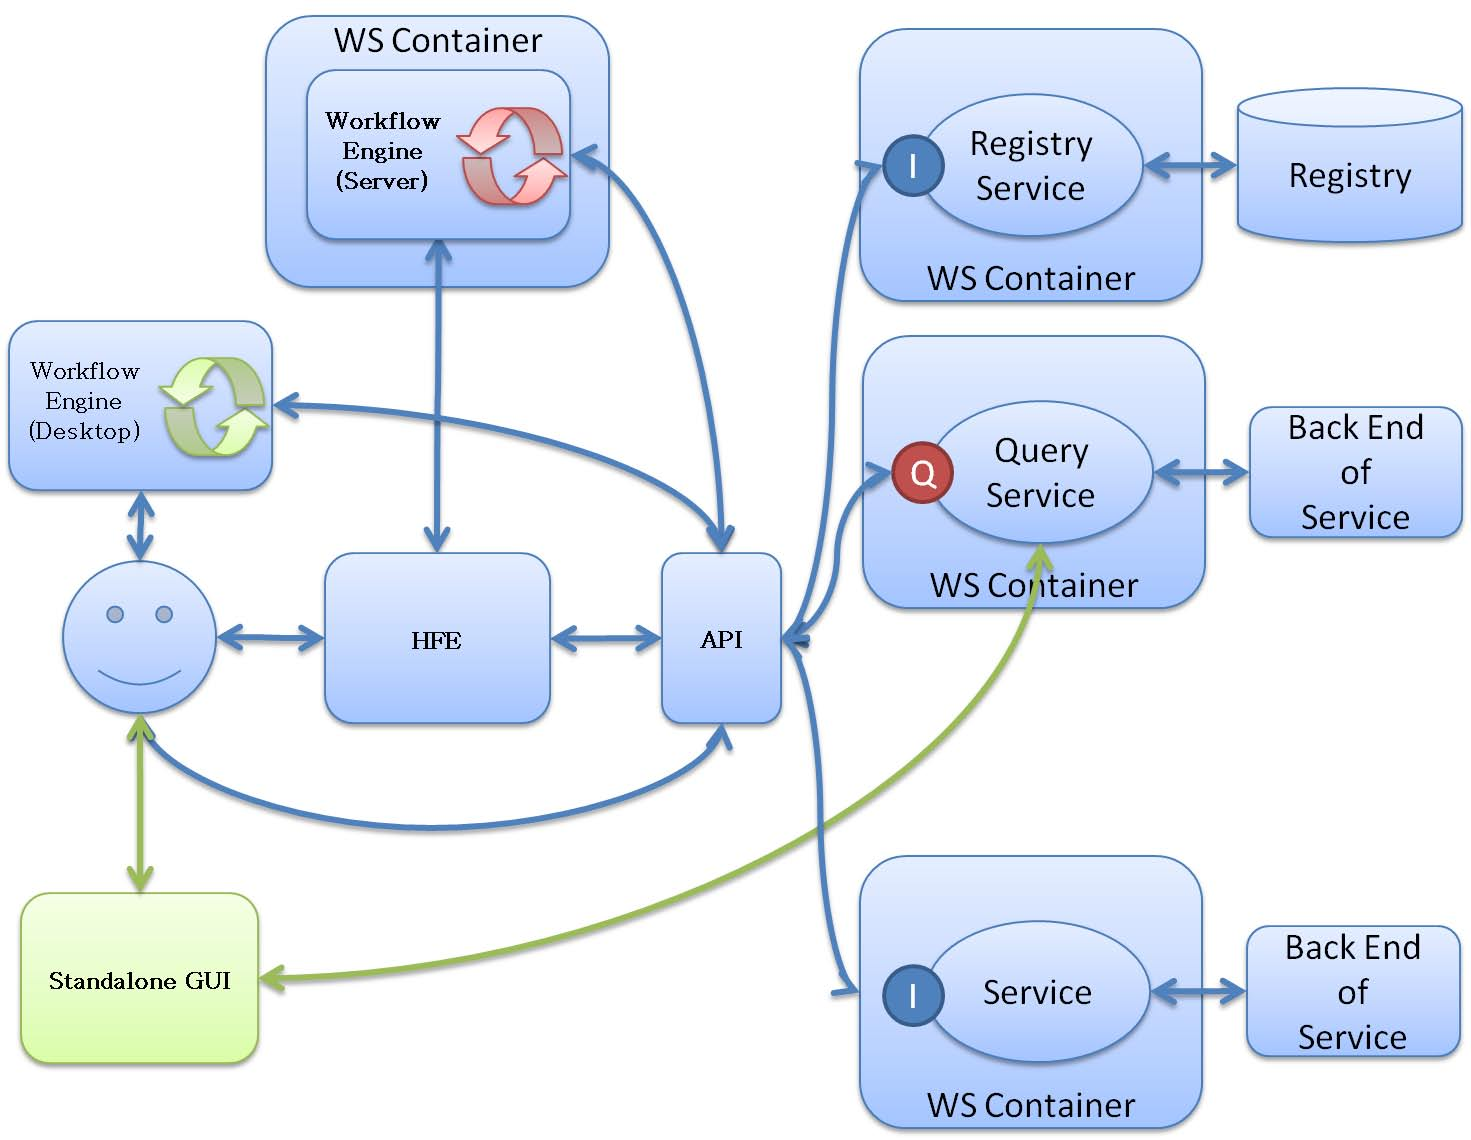
\includegraphics[width=3in]{HELIO-Architecture-Detail.pdf}
\caption{General architecture of the HELIO infrastructure}
\label{arch.detail}
\end{figure}

Figure~\ref{arch.detail} also comprehends three representative examples of HELIO services. 

\begin{itemize}
\item{The \emph{Registry Service}. The Registry Service, along with the Monitoring Service (not shown in Figure~\ref{arch.detail}) is a fundamental part of the architecture as it allows the discovery of all the instances of the services}
\item{A \emph{Helio Query Service}. Some of the HELIO services perform queries on catalogues of data and metadata. As these services show several similarities a single query interface that use VOTables (TODO: Kevin, Vineeth: Any references to VOTables ?) has been developed. This query interface is further detailed in section~\ref{arch.queryservice}}
\item{A \emph{Generic HELIO Service}}
\end{itemize}

\subsubsection{The HELIO Query service}
\label{arch.queryservice}
TODO : Vineeth, Kevin : 1/3 of a page with the details of the HELIO query service

\subsubsection{The HELIO API}
\label{arch.api}
TODO : Marco : 1/3 a page with the details of the  API

\subsubsection{HELIO and Taverna}
\label{arch.taverna}
TODO : Donal : 1/3 a page with the details of TAVERNA in HELIO

\subsection{Subsection Heading Here}
Subsection text here.
\subsubsection{Subsubsection Heading Here}
Subsubsection text here.
